\chapter{Experimenty}\label{chap:experiments}

V~tejto kapitole porovnáme jednotlivé typy architektúr neurónových sietí, porovnáme ich úspešnosť a ukážeme, ktorá z~nich je najvhodnejšia. Ďalej sa budeme venovať aj predspracovaniu segmentov, ktoré priamo ovplyvňuje vlastnosti trénovania a úspešnosť sietí.
\bigskip

\section{Trénovanie}

Trénovanie dopredných sietí sme robili pomocou algoritmu \textit{Backpropagation} - algoritmu spätného šírenia chyby \cite{haykin1999neural}. Sieti sme postupne predkladali dáta s~informáciou či sa jedná o~ruku alebo nie. Pred každou epochou sme dáta náhodne preusporiadali. 

Pri rekurentných sieťach sme predkladali postupnosti dát, pričom sme zachovávali poradie obrázkov v~postupnosti. Rekurentné vstupy sme updatli len v~prípade, že sme detekovali ruku. Po každej postupnosti sme rekurentné vstupy resetli na 0. Takto simulujeme správanie siete v~reálnej aplikácii.

\section{Testovanie a vyhodnocovanie neurónových sietí}
Pri trénovaní sa snažíme minimalizovať kvadratickú chybu. Preto aj pri vyhodnocovaní úspešnosti sietí budeme používať túto metriku.

Kvadratická chyba sa počíta takto: $$\frac{1}{2}(t-o)^2$$
$t$ je cieľová hodnota a $o$ je výstup siete. V~tabuľkách budeme uvádzať priemernú kvadratickú chybu, ktorú budeme počítať ako súčet všetkých kvadratických chýb deleno počet testovacích vstupov. 

\section{Trénovacie a testovacie dáta}

Na generovanie dát sme použili upravenú verziu našej aplikácie (kapitola \ref{chap:neuralnetapp}), ktorá umožňovala ukladanie vysegmentovaných obrázkov na disk bez toho, aby došlo k~výraznému spomaleniu. 

Trénovacie dáta sme rozdelili na dve sady. Každá sada bola rozdelená na trénovaciu a testovaciu množinu.

Prvou sadou sme vyhodnocovali vlastnosti rôznych typov architektúr neurónových sietí a vplyv fourierovej transformácie. Obsahovala dáta, ktoré boli rozdelené do postupností. To nám umožňovalo trénovať nimi rekurentné neurónové siete. Dopredné siete tieto dáta brali ako jednotlivé obrázky. Na jednu postupnosť pripadá v~priemere cca 11 obrázkov.

Druhá sada bola špecializovaná na vyhodnocovanie použitia pôvodného vs. rozdielového obrázka. Z~tejto sady boli vyňaté obrázky rúk, ktoré sa nepodarilo algoritmu floodfill správne vyselektovať. Porovnávali sme teda úspešnosti v~ideálnych prípadoch.

\begin{table}[h]
\catcode`\-=12 %kvoli babelu a pomlcke
\centering
\begin{tabular}{|l|c|c|c|c|c|}
\cline{2-5}
\multicolumn{1}{l}{} & \multicolumn{2}{|c|}{\textbf{Testovacia množina}} & \multicolumn{2}{c|}{\textbf{Trénovacia množina}}\\ 
\hline
\textbf{Sada} & \textbf{ruky} & \textbf{ostatné} & \textbf{ruky} & \textbf{ostatné} \\ \hline
1. sada & & & & \\ \hline
2. sada & & & & \\ 
\hline
\end{tabular}
\caption{Veľkosti sád vstupov}
\label{tab:neuroncountcmp}
\end{table}

%Na trénovanie sme použili dáta fourierovych transformácií (viď \ref{sect:ft}). Množina dát obsahovala cca 800 vzorov, ktoré boli pri trénovaní rekurentnej neurónovej siete rozdelené do približne 70 postupností.

%Na testovanie sme mali množinu cca 650 vzorov (60 postupností), ktoré sme nepoužívali na trénovanie.

\section{Porovnanie architektúr neurónových sietí}


Experimentálne sme zistili, že dvojvrstvová sieť na tento problém stačí a tretia vrstva nepomáha.

% - 3vrstvovú sieť sa nám ani nepodarilo natrénovať 
{\color{red}
V~tabuľke \ref{tab:neuroncountcmp} je porovnanie úspešnosti na testovacích dátach pre rôzne počty neurónov a priemerná kvadratická chyba.
}

\begin{table}[h]
\catcode`\-=12 %kvoli babelu a pomlcke
\centering
\begin{tabular}{|l|c|c|c|c|c|}
\cline{2-5}
\multicolumn{1}{l}{} & \multicolumn{2}{|c|}{\textbf{Testovacia množina}} & \multicolumn{2}{c|}{\textbf{Trénovacia množina}} & \multicolumn{1}{l}{}\\ 
\hline
\textbf{Počet neurónov} & \textbf{úspešnosť} & \textbf{chyba} & \textbf{úspešnosť} & \textbf{chyba} & \textbf{čas} \\ \hline
40 & 81,11\% & 0,0818 & & &\\ \hline
45 & 85.55\% & 0,0643 & & &\\ \hline
50 & 85,19\% & 0,0667 & & &\\ \hline
60 & 85,19\% & 0,0634 & & &\\ 
\hline
\end{tabular}
\caption{Porovnanie úspešnosti NS pri rôznych počtoch neurónov}
\label{tab:neuroncountcmp}
\end{table}

%\subsection{Viac vrstvová dopredná neurónová sieť - upravená verzia}

%\begin{figure}[h]
%  \begin{center}
%    \includegraphics[width=0.3\textwidth]{images/dffnn}
%  \end{center}
%  \caption{Upravená dopredná neurónová sieť}
%  \label{fig:dffnn}
%\end{figure}

%V upravenej verzii sme upravili spodnú vrstvu siete - tú, ktorá dostáva vstup. Vstup je rozdelený na 16 častí a ku každej časti je pridelených niekoľko neurónov. Každý neurón spracúva len vstupy z jeho časti (obr. \ref{fig:dffnn}). 

%Jej výhodou je rýchlosť. Náš vstup má rozmer $128\times 128 = 16384$, čo nie je malé číslo. Rozdelíme ho na 16 častí s veľkosťou $32\times 32 = 1024$. Takto namiesto toho aby každý vstupný neurón počítal s 16384 vstupmi počíta len s 1024, čo je $16\times$ rýchlejšie. Skupina neurónov pridelená danej časti sa stará len o príznaky zo svojej časti a nie je ovplyvňovaná ostatnými časťami. 

%Nevýhodou je to, že neuróny sú fixne pridelené na jednotlivé vstupy. V pôvodnej sieti si neuróny sami vyberali, ktoré časti vstupu sú pre nich najvýznamnejšie a mohli tak lepšie pokryť vstup.

\begin{table}[h]
\catcode`\-=12 %kvoli babelu a pomlcke
\centering
\begin{tabular}{|l|c|c|c|c|c|}
\cline{2-5}
\multicolumn{1}{l}{} & \multicolumn{2}{|c|}{\textbf{Testovacia množina}} & \multicolumn{2}{c|}{\textbf{Trénovacia množina}} & \multicolumn{1}{l}{}\\ 
\hline
\textbf{Počet neurónov} & \textbf{úspešnosť} & \textbf{chyba} & \textbf{úspešnosť} & \textbf{chyba} & \textbf{čas} \\ \hline
48; 12 & 83,33\% & 0,0745 & & &\\ \hline
112; 12 & 84,07\% & 0,0714 & & &\\
\hline
\end{tabular}
\caption{Porovnanie úspešnosti upravenej NS pri rôznych počtoch neurónov}
\label{tab:neuroncountcmp2}
\end{table}

{\color{red} Keď si porovnáme tabuľku \ref{tab:neuroncountcmp2} s~tabuľkou \ref{tab:neuroncountcmp} zistíme, že rozdiel v~úspešnosti nie je veľký. Preto sme sa rozhodli, že použijeme radšej túto architektúru. Trénovanie aj klasifikácia je značne rýchlejšia.}
%TODO popisat aj pocty pouzitych neuronou 
%TODO trenovacie data do tabuliek

\todo

%\subsection{Rekurentná neurónová sieť}

%Architektúra našej rekurentnej neurónovej siete vychádza z upravenej doprednej neurónovej siete, s tým, že namiesto obyčajného neurónu používame v niektorej vrstve rekurentný neurón (obr. \ref{fig:recurentneuron}). Viac o tomto type siete nájdete v kapitole \ref{chap:rnn}.

\begin{table}[h]
\catcode`\-=12 %kvoli babelu a pomlcke
\centering
\begin{tabular}{|l|c|c|c|c|c|}
\cline{2-5}
\multicolumn{1}{l}{} & \multicolumn{2}{|c|}{\textbf{Testovacia množina}} & \multicolumn{2}{c|}{\textbf{Trénovacia množina}} & \multicolumn{1}{l}{}\\ 
\hline
\textbf{Rekurentná vrstva} & \textbf{úspešnosť} & \textbf{chyba} & \textbf{úspešnosť} & \textbf{chyba} & \textbf{čas} \\ \hline
spodná & 83,33\% & 0,0745 & & &\\ \hline
\end{tabular}
\caption{Porovnanie úspešnosti rekurentnej NS pri rôznom umiestnení rekurencie}
\label{tab:neuroncountcmp2}
\end{table}

\todo
%end NeuralNet

%\section{Metódy na zlepšenie úspešnosti klasifikátora ruky}
%\label{sect:metodyzlepseniaklasifikacie}

%V tejto časti sa budeme zaoberať jednotlivými segmentami, ktoré budeme predkladať neurónovej sieti, aby nám povedala, či je to ruka, alebo nie.

%\subsection{Trénovacia a testovacia množina}
%\todo 

%\subsection{Normalizácia dát} %TODO Dat inde? asi nie
%Ideálne vstupy pre neurónovú sieť sú z intervalu $\langle 0,1\rangle$. Pixle čiernobielych obrázkov majú hodnoty $\{0\dots 255\}$. Pri obrázkoch zvolíme pre farbu pozadia hodnotu 0 a pre objekt ostatné hodnoty. Z tohto dôvodu chceme, aby rozdiel v normalizovanej hodnote medzi 0 a 1 bol najväčší a postupne klesal. Preto sme za normalizačnú funkciu zvolili:

%$$f(x)=\frac{1}{1+x}$$

%Pre normalizáciu fourierovej transformácie sme zvolili tú istú funkciu. %TODO dôvod? 

%TODO Popisat preco je to nutne a v com to pomaha

%\todo 

\section{Porovnanie rôznych typov dát}
%Nevýhodou rozdielového obrázka je, že zmena spôsobená pohybom sa v ňom vyskytne dvakrát. Raz na mieste, kam sa objekt posunul a raz na mieste odkiaľ sa posunul. Toto sme chceli eliminovať tak, že sa vyberie ruka z pôvodného obrázka podľa farby. Táto ruka tam bude vždy len raz. Bohužiaľ tento prístup mal viac zlých vlastností ako dobrých.

%Pri vyberaní obrázka treba mať nastavené správne parametre, podľa ktorých sa rozhoduje čo pridať do výberu a čo nie. Tieto parametre veľmi závisia od osvetlenia. Navyše osvetlenie sa môže meniť pri pohybe ruky, čo veľmi stažuje nastavenie správnych parametrov. Pred použitím aplikácie by sa aplikácia musela nakalibrovať, čo znižuje komfort jej použitia.

%Ďalší problém je správne tipnúť bod, ktorý patrí ruke, aby sa z neho mohla odštartovať selekcia. Pokiaľ by bola v danom obdĺžniku len dlaň, tak nie je až také ťažké sa správne trafiť - je takmer isté, že kúsok pod stredom obrázka bude dlaň. Bohužiaľ často sa stane, že užívaťeľ pohne nielen rukou, ale aj predlaktím a segmentačný algoritmus zaradí do segmentu aj predlaktie. Potom sa môže stať, že bod ruky netrafíme.

%{\color{red}
%Rozhodujúcim problémom však bolo to, že úspešnosť siete na dátach, ktoré ani neobsahovali zle vybraté ruky bola aj tak nižšia ako u rozdielového obrázka (tabuľka \ref{tab:neuraldatacmp}). Preto sme sa rozhodli radšej pridať ďalšie dáta do trénovacej množiny pre rozdielové obrázky. Pri vyhodnocovaní tejto časti sme použili menšiu trénovaciu a testovaciu sadu, ktorá obsahovala cca 350 trénovacích a 300 testovacích vzorov. Sada neobsahovala zle vybraté ruky.
%}

%\subsection{Fourierova transformácia} \label{sect:ft}
%Fourierova transformácia zvykne často pomáhať, keď sa použie na predspracovanie dát pri trénovaní obrazových alebo zvukových vzoriek. Preto sme sa aj my rozhodli vyskúšať aký bude mať vplyv na úspešnosť.

%Fourierova transformácia bola použitá na segment ako celok, potom bola prevedená do reálnych čísel ako absolútna hodnota z komplexného čísla a následne normalizovaná.

%Konvergencia chyby pri trénovaní bola značne rýchlejšia a použitie transformácie umožnilo dosiahnuť menšiu chybu na trénovacej množine. 

%TODO
%Úspešnosť na testovacej množine bola mierne nižšia.
%\todo

\begin{table}[h]
\catcode`\-=12 %kvoli babelu a pomlcke
\centering
\begin{tabular}{|l|c|c|c|c|c|}
\cline{2-5}
\multicolumn{1}{l}{} & \multicolumn{2}{|c|}{\textbf{Testovacia množina}} & \multicolumn{2}{c|}{\textbf{Trénovacia množina}} & \multicolumn{1}{l}{}\\ 
\hline
\textbf{Typ dát} & \textbf{úspešnosť} & \textbf{chyba} & \textbf{úspešnosť} & \textbf{chyba} & \textbf{čas} \\ \hline
\textbf{Rozdielový obr.} & 83,33\% & 0,0745 & & & \\ \hline
\textbf{Pôvodný obr.} & 68,52\% & 0,1174& & &\\ \hline
\textbf{Rozdielový -- FT} & 75,18\%& 0,0895& & &\\ \hline
\textbf{Pôvodný -- FT} & 70.37\%& 0,1158& & &\\
\hline
\end{tabular}
\caption{Porovnanie úspešnosti NS pri rôznych dátach}
\label{tab:neuraldatacmp}
\end{table}